\section{Background}
%
\begin{frame}
    \frametitle{Device Mapper Cache}
    \begin{block}{What is it?}
	A generic block-level caching mechanism
	for storage networks
    \end{block}
    \vspace{2ex}
    \begin{block}{What does it do?}
	Cache popular data locally to reduce
	network and storage server latency
    \end{block}
    \vspace{2ex}
    \begin{block}{How does it work?}
	Built upon the Linux kernel device mapper, which
	maintains the mapping between a source device, and
	a cache device.
    \end{block}
\end{frame}
\begin{frame}
    \frametitle{Device Mapper Cache}
    \begin{tabular}{m{0.465\linewidth}m{0.465\linewidth}}
	%\hline
	DM Cache takes advantage of spatial and temporal
	locality by caching data locally and using LRU for
	cache replacement. &
	\begin{figure}
	    %\caption{Device Mapper Layout}
	    \centering 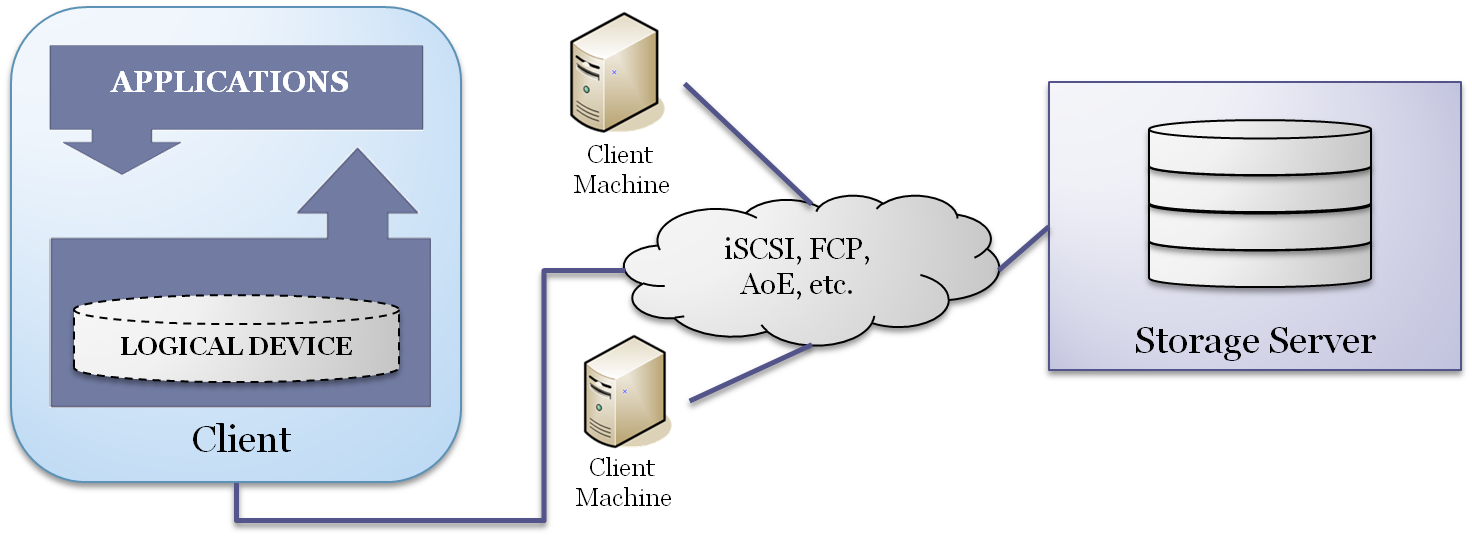
\includegraphics[scale=.23]{current.png}
	    \label{fig:dm}
	\end{figure} \\
	%\hline
    \end{tabular}
    \begin{block}{Device Mapper Cache}
	\begin{itemize}
	    \item Distributed shared storage systems (SAN, iSCSI, AoE, \&c.)
		support better scalibility by using block-level caching
		on the client side
	    \item Fast mass storage devices, like Solid State Drives (SSDs) 
		are excellent candidates for cache devices
	    \item While DRAM can increase throughput by
		supporting more IOPS, SSD caches provide greater capacity
	\end{itemize}
    \end{block}
\end{frame}
\begin{frame}
    \frametitle{Replication}
    One-to-many distribution of data from a \textit{source}
    to several \textit{targets} to hold replicas of original data
    \begin{block}{Pessimistic Replication}
	\begin{itemize}
	    \item synchronous
	    \item consistent, but not optimal: system may incur
		performance bottleneck from unpredictable network
		and storage latency
	    \item low availability: replicator will block until data is
		fully propagated to all targets
	\end{itemize}
    \end{block}
    \begin{block}{Optimistic Replication}
	\begin{itemize}
	    \item asynchronous
	    \item high availability, low latency, not consistent
	    \item less reliable than pessimistic replication
	\end{itemize}
    \end{block}
\end{frame}
\begin{frame}
    \frametitle{Cooperative Caching}
    \begin{block}{Basic Idea}
    	\begin{itemize}
	    \item Collaboration across a network in order to saturate
		the space that is available for caching
	    \item Use IP-based interface for cache devices to communicate
	\end{itemize}
    \end{block}
    \begin{block}{Sub-optimal Implementation}
	Use iSCSI. Works at the block layer. Only need a logical cache
	partition to hold replicas.
    \end{block}
    \begin{block}{Better Implementation}
	Have kernel modules interact at the block layer through TCP
	protocol. iSCSI network interface adds unnecessary file system
	indirection.
    \end{block}
\end{frame}
